\documentclass[12pt,oneside]{amsbook}
\usepackage[utf8]{inputenc}
\renewcommand{\baselinestretch}{2}
\usepackage[utf8]{inputenc}

\numberwithin{equation}{chapter}
% This numbers the equations within each chapter as 1.1, 1.2, 2.1, etc.
\numberwithin{figure}{chapter}
\numberwithin{section}{chapter}
\usepackage{tikz}
\usetikzlibrary{arrows}
\usepackage{graphicx}

\newtheorem{thm}{Theorem}[chapter]
\newtheorem{lemma}[thm]{Lemma}
\newtheorem{prop}[thm]{Proposition}
\newtheorem{corollary}[thm]{Corollary}

\newenvironment{defn}[1][Definition]{\begin{trivlist}
\item[\hskip \labelsep {\bfseries #1}]}{\end{trivlist}}

\newcommand{\R}{\mathbb{R}}
\newcommand{\T}{\mathcal{T}}
\newcommand{\B}{\mathbb{B}}
\newcommand{\n}{$n$}
\newcommand{\Y}{\Gamma_Y}
\newcommand{\C}{$C^2(\Y)$}


\begin{document}
\frontmatter % Pages here will be numbered with Roman numerals.
\title[]{Collision Avoidance on Finite Graphs}
\author{Tynan Flawn Sailor Daly}
\address{Department of Mathematics\\Bates College\\Lewiston, ME 04240}
\date{December 12, 2014}
\maketitle

\newpage
\thispagestyle{empty}
% THESIS COVER PAGE

% Choose Honors/Senior and Arts/Science below as appropriate.

\vspace*{4cm} 
% LaTeX will remove blank space at the start or end of a page,
%   but the asterisk prevents this.

\centerline{\LARGE \textbf{Collision Avoidance on Finite Graphs}}
%\centerline{\LARGE \textbf{Topology and Stuff}}
\bigskip\bigskip
\centerline{\Large  A One Semester Thesis}
%\centerline{\Large  A Senior Thesis}
\medskip
\centerline{\Large Presented to the Department of Mathematics}
\medskip
\centerline{\Large Bates College}
\medskip
\centerline{\Large in partial fulfillment of the requirements for the}
\medskip
\centerline{\Large Degree of Bachelor of Arts}
%\centerline{\Large Degree of Bachelor of Science}
\medskip
\centerline{\Large by}
\medskip
\centerline{\Large Tynan Flawn Sailor Daly}
\medskip
\centerline{\Large Lewiston, Maine}
\medskip
\centerline{\Large December 12, 2014}

\newpage


\setcounter{page}{2}

\tableofcontents
 \listoffigures

\chapter*{Acknowledgments}
% The asterisk prevents this file from being labelled
% as a 'chapter.'

I would like to begin by thanking my thesis advisor, Professor Pallavi Jayawant for not only pushing me to be a better mathematician, but also for believing in me. This has been a truly wonderful experience. Thank you for sharing it with me.\\

My major advisor, Professor Chip Ross, in whose class I first experience the thrill of solving a proof and the sublime beauty of mathematics.\\

My roommates Jordana Gluckow and Jake Barbato for catching typos, bringing me food from Commons, and listening to me drone on endlessly about my thesis.\\

Eric Towne and Will Ash, without whom I could not have recovered my corrupted files.\\

My friends Ben Gilmore, Arnaud Cluzel, Matthew Neal, Maxwell Goldfarb, Darnell Morrow, Ali Hakasui, Alex Donatelle, Charlie McKitrick, Hannah Kiesler, and the Men's Water Polo Team for their constant love and support.\\

Finally, I would like to thank my family; Mom, Dad, Shane, and Emme. I love you all.            % Acknowledgments
\mainmatter
\chapter{Introduction}
\section{The Setting: Robots in Industry}
As a result of recent technological advances, robotic engineers, mathematicians, and computer scientists have witnessed a proliferation of robotics across a wide range of industrial applications. Robots are generally employed in this matter to complete tasks which humans cannot, and so are highly specialized and expensive. In order to carry out tasks, robots are often required to move around a workspace; however, robots are fragile and so collisions result in costly repairs and extensive downtime.

Robotic movement can be broadly defined into two categories: restricted and unrestricted movement. Robots with restricted movement capabilities have fixed movement networks, such as wires or tracks which connect different stations in a workspace. Robots whose movements are unrestricted however, have access to a full degree of movement. While robots with an unrestricted movement network may be more ubiquitous in the public mind, their initial and subsequent maintenance costs are significant, and so robots with fixed movement networks are utilized to a higher degree. 

While these movement networks may be simple to visually illustrate, the set of all possible robot configurations, which we call the configuration space, is typically not. We often find configuration spaces defy our ability to graphically conceptualize due to the fact that they exist in extremely high dimensions. Furthermore, the complexity of their dimension grows linearly with each additional robot added.

This problem of dimensional complexity also poses problems for finding collision-free movement schemes. In order to determine the optimal schedule for robotic movement, robotic engineers often employ graph algorithms to find safe movement patterns, however, the complexity of configuration spaces often renders these algorithms increasingly inefficient as movement networks become more complicated.

Thus the problem is this: Given $N$ named robots on a movement network $\Gamma$ with a configuration space $C^N(\Gamma)$, how can we simplify the configuration space in order to apply graph algorithms?

\section{Contributions of this Thesis}
This thesis expands upon the work done by A. Abrams in his thesis \cite{thesis}, which is summarized in an article he coauthored with R. Ghrist \cite{factory}. The article presents a summary of their work, but spares a significant number of details. Abram's thesis, however, requires a deep background in algebraic topology. This work will serve as a bridge between these two texts.

In order to establish the mathematical framework to discuss the problem, chapter 2 will serve as an introduction to topics of graph theory and topology, and then proceed to introduce a bridge between these two fields. This chapter is by no means an exhaustive text of either subject, but offers a useful survey of the relevant concepts. The remainder of this thesis will devote itself to the creation of and discretization from an example fixed movement network. Chapter 3 will explicitly construct a movement space in order to find the configuration space. We will then describe the discretization process in chapter 4. The paper will conclude by discussing theorems about when the techniques examined in chapters 3 and 4 can be safely applied.

While building and discretizing the configuration space for the specific example provided in chapters 3 and 4 may prove valuable, we hope that readers use this work as a lesson for how techniques presented here can be generally applied.
   			% Introduction 

\chapter{Chapter Zero}
We begin, not by discussing the movement of robots, but by laying out the tools needed to fully understand the problem at hand. The problem we are investigating exists in graphs, but uses topological tools to find solutions. The first two sections of the chapter serve to establish a sufficient mathematical base with which we may study the problem of autonomous movement along fixed paths.

The first section will focus on the basics of graph theory and the second will do so similarly with topology. The third extends ideas from the preceding sections in order to bridge the gap between our two primary fields of focus.

\section{Graphs}\label{sec:graphs}
%\textit{Ty's note: This section needs more comprehensive citing.}

We begin by exploring some basic elements of graph theory. A graph is a one-dimensional mathematical structure composed of edges and nodes. While graphs may be either finite or infinite, our attention will be directed at finite graphs.

\begin{defn}
A graph $G$ is the pair $G=(V,E)$ of vertices $V(G)$, usually denoted through letters or numbers, and edges $E(G)$. We say a vertex is a point in the graph and an edge is an unordered pair of vertices in $V(G)$\cite{ed}. 
\end{defn}

Graphs are useful in understanding the relationship between objects. As a result, they are used to model public transit systems, infectious diseases, communication networks, and countless other things. Since our focus is on robots which move around on a graph, let us choose to use a public transit system, specifically a railway system, as a running example.

\begin{figure}[h!]
\caption{The Graph $G$ of a Rail System}\label{fig:railgraph}
\centering
\begin{tikzpicture}
  [scale=.7,auto=left,every node/.style={circle,fill=blue!30}]
  \node (n1) {a};
  \node (n2) [above right of=n1]    {$b$};
  \node (n3) [above left of=n1]     {$c$};
  \node (n4) [below of=n1]          {$d$};
  \node (n5) [above left of=n2]     {$e$};
  \node (n6) [above right of=n5]    {$f$};
  \node (n7) [right of=n6]          {$g$};
  \node (n8) [below left of=n4]     {$h$};
  \node (n9) [below right of=n4]    {$i$};
  
    
\foreach \from/\to in
{n1/n3,n2/n1,n4/n1, n2/n5, n2/n6, n6/n7, n4/n8, n4/n9}
    \draw (\from) -> (\to);
\end{tikzpicture}
\end{figure}

Consider a train system consisting of train stations and the track which connects them. It may seem obvious then to construct a graph of some arbitrary railway system by representing nodes as stations and the tracks between them as edges. Consider the example in Figure~\ref{fig:railgraph}. Here we have a graph of a rail system with stations denoted by lettered vertices and the tracks as edges.

As we can see, our graph contains little information of physical routes traveled by trains, as each station is seemingly equidistant from one another but in actuality may be an hour or several minutes away, but the information needed as to how to effectively travel from one station to another is preserved by the relationship between edges and vertices. Even though we do not know the actual distance or time involved, it is clear from our graph that station $b$ is only one stop away from station $a$. In this case we say that $a$ and $b$ are \textbf{adjacent}.

\begin{defn}
We say that $v_x,v_y\in V(G)$ are adjacent if there exists some $e\in E(G)$ such that $e$ \textit{joins}, or connects, $v_x$ and $v_y$. Two edges are \textbf{incident} if they share a common vertex. A graph is \textbf{simple} if no two edges are incident to the same two vertices and no vertex is \textbf{adjacent} to itself.\cite{ed}
\end{defn}

\begin{figure}[h]
\centering
\caption{Not Simple and Simple Graphs}
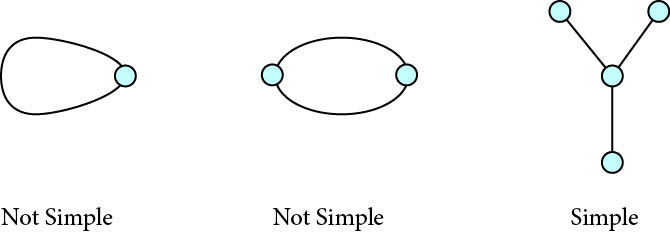
\includegraphics[scale=.5]{simples.jpg}
\label{fig:simple}
\end{figure}

In simple graphs, \textbf{degree} of a vertex $v\in V(G)$, denoted as deg$(v)$, is the number of vertices adjacent to $v$. Looking at the graph in Figure~\ref{fig:simple}, we can see that deg$(a)=3$ while deg$(f)=2$. We can classify a vertex $v$ as \textbf{essential} if deg$(v)\neq 2$. Conversely, we say vertices with degree two are \textbf{non-essential}\cite{ed}.

We define a \textbf{path} as a sequence of adjacent vertices along their incident edges such that no vertex or edge is repeated. We denote a path from $v_0$, the \textit{initial vertex}, to $v_k$, the \textit{terminal vertex}, as $(v_0,v_k)\text{-path }=v_0,e_0v_1,e_1\dots,e_{k-1},v_k$ \cite{ed}. In an abuse of notation, it is common to exclude edges from our sequence for simple graphs. A path containing $n$ vertices has length $k=n-1$.


We say a graph is \textbf{connected} if, for every $v_x,v_y \in V(G)$, there exists a path such that $v_x,v_{x+1},\dots, v_{k}=v_y$\cite{ed}. The graph in Figure \ref{fig:railgraph} is a connected graph, but it will not be if any of the edges are removed. Figure~\ref{fig:connected} shows a disconnected subgraph of the graph G from Figure~\ref{fig:railgraph}.

\begin{figure}[h]
\centering
\caption{A Disconnected Subgraph of $G$}
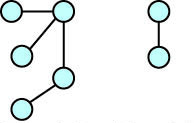
\includegraphics[scale=.5]{connected.jpg}
\label{fig:connected}
\end{figure}

For connected graphs, we can use the length of a path to define an informal metric, called the shortest path metric, defined as the path where $k$ is minimized. If we again return to Figure~\ref{fig:railgraph}, we see that the path from $g$ to $a$ is $g,f,b,a$ is shorter than the path from $d$ to $a$, which is $d, a$.

A cycle is a path such that the initial and terminal vertices are the same and no edges or vertices are repeated. Figure \ref{fig:railgraph} contains no cycles while the middle graph in Figure~\ref{fig:simple} does contain a cycle.



We can employ our understanding of a graph's paths to further classify graphs. We say a graph, such as the graph in Figure~\ref{fig:tree}, is a \textbf{tree} if it is connected and has no cycles \cite{ed}. The sub-graph of $G(V,E)$ formed by $a,b,c,$ and $d$ and their incident edges is a tree.

\begin{figure}[h]
\caption{The Tree which is a Subgraph of G}\label{fig:tree}
\centering
\begin{tikzpicture}
  [scale=.7,auto=left,every node/.style={circle,fill=blue!30}]
  \node (n1) {a};
  \node (n2) [above right of=n1]  {b};
  \node (n3) [above left of=n1] {c};
  \node (n4) [below of=n1] {d};

\foreach \from/\to in
{n1/n3,n2/n1,n4/n1}
    \draw (\from) -> (\to);
\end{tikzpicture}
\end{figure}


We use graphs to represent relationships between objects, but in order manipulate these relations we will need to incorporate ideas from topology.


\section{Topology}\label{sec:topology}
Topology may be broadly defined as the study of abstract mathematical space. In Section \ref{sec:graphs} we restricted ourselves to characterizing one-dimensional space, but the concepts in topology will free us from such restrictions. 

\subsection{Topological Spaces}

We begin our discussion of topology by defining a topological space.
\begin{defn}
Let $X$ be a set. We define a topology $\mathcal{T}$ on $X$ to be a collection of subsets of $X$, called open sets, such that
\begin{enumerate}
\item $X$ and $\emptyset$ are elements of $\mathcal{T}$;\
\item the union of any collection of subsets in $\T$ belongs to $\T$;\
\item the intersection of finitely many subsets in $\T$ belongs to $\T$.
\end{enumerate}
We say a set $X$, together with a topology on it, is a topological space.
\end{defn}


Formally, we define a topological space to be a space with a topology on it, $(X,\mathcal{T})$, but it is a common practice to simply say $X$ with the understanding there is a topology on it.

Let us start with a simple example, namely the finite set $X=\{1,2,3\}$. Now let us define a topology on $X$. Let $\mathcal{T}_0=\{X,\emptyset\}$. Clearly this meets the definition of a topology. We call this topology the \textit{trivial topology}. Let $X$ be the set defined above, but now let $\mathcal{T}_1=\{\emptyset, \{2\}, \{2,3\}, X\}$. This is an example of a non-trivial topology on $X$. Let us take a moment to compare the two topologies we have just constructed. Notice that $\mathcal{T}_0 \subseteq \mathcal{T}_1$. We say that $\mathcal{T}_0$ is \textbf{coarser}, or weaker, than $\mathcal{T}_1$. Similarly we say $\mathcal{T}_1$ is \textbf{finer} or stronger than $\mathcal{T}_0$. 

We can also define a topology on $\R$. Consider the collection $\mathcal{T}$ of subsets $U$ such that for every $x \in U$ there exists an $\epsilon >0$ such that $(x-\epsilon, x+\epsilon)\subset U$. We will now show this collection to be a topology.


\begin{proof}
We begin by showing that $\emptyset$ is in $\mathcal{T}$. Since there is no $x \in \emptyset$, there does not need to be an $\epsilon >0$, and so it is open. It is also clear to see that by definition $\R$ is open since for every $x$ in $\R$, there is an $\epsilon >0$ such that $(x-\epsilon, x+\epsilon) \subset \R$.

Let $U,V \subset \R$ be in $\T$ and let $W = U \cap V$. If $U$ and $V$ do not intersect, then $W=\emptyset$, which is an element of $\mathcal{T}$. Thus assume $W\neq \emptyset$. Let $x \in W$. Since $x$ is in $U$, there exists $\epsilon>0$ such that $(x-\epsilon, x+\epsilon)\subset U$ and since $x$ is in $V$ there exists $\delta>0$ such that $(x-\delta, x+\delta)\subset V$. Without loss of generality, assume that $\delta \leq \epsilon$. It follows that $(x-\delta, x+\delta) \subseteq (x-\epsilon, x+\epsilon) \subset U$. Thus $(x-\delta, x+\delta)\subset U \cap V = W$, so $U\cap V$ is an open set. For finite intersections of three or more subsets of $\R$, an inductive argument can be made.

To finish the proof we will show that the union of any collection of open sets is open. Let $A=\bigcup_{i\in I} U_i$ where ${U_i}$ is a collection of open sets in $\R$ and $i$ belongs to some index set $I$. Let $x \in A$. So there exists some $i\in I$ such that $x\in U_i$, and so there exists some $\epsilon $ such that $(x-\epsilon,x+\epsilon)\subset U_i \subseteq  \bigcup_{i\in I} U_i = A$. Thus the union of any collection of subsets in $\mathcal{T}$ belongs to $\mathcal{T}$.

Since the collection of open sets $\T$ satisfies all three conditions of a topology, $\T$ is a topology on $\R$. 
\end{proof}

We say this particular $\T$ is the standard topology on $\R$. 

The previous proof demonstrated the construction of the standard topology on the real line, but what we did not mention is that the open sets $U$ are \textbf{neighborhoods} of points in them.  

\begin{defn}
Let $X$ be a topological space and $x\in X$. An open set $U$ containing $x$ is said to be a neighborhood of $x$.
\end{defn}


This is a powerful definition, principally because it helps us determine if a set is open or not, which will aid us as we explore topology in greater depth.

In the proof above we showed the entire collection of open sets satisfied the definition for a topology. This may seem intuitive for familiar spaces such as $\R$, but for less familiar or more complicated spaces it may be more challenging. Instead, we can define a smaller collection of open sets called a \textbf{basis} and then use it to generate the remaining open sets in the topology.

\begin{defn}
Let $X$ be a set and let $\mathbb{B}$ be a collection of subsets of $X$. The collection $\mathbb{B}$ is a basis for a topology on $X$ if the following conditions are satisfied:
\begin{enumerate}
\item for $x\in X$ there exists some $B\in \mathbb{B}$ such that $x\in B$.
\item if \textbf{basis elements} $B_1, B_2 \in \mathbb{B}$ and $x\in B_1 \cap B_2$, there exists some $B_3$ such that $x \in B_3 \subseteq B_1 \cap B_2$.\cite{top}
\end{enumerate}
\end{defn}

Simply put, every element in $X$ is in a basis element and every element in the intersection of two basis elements is contained in a basis element which is a subset of the intersection.

Having examined the definition of a basis, we are now free to use it in defining a topology on a set.

\begin{defn}
Let $\B$ be a basis on $X$. The \textbf{topology $\T$ generated by $\B$} is obtained by defining the open sets to be the empty set and every set equal to the union of basis elements.
\end{defn}

Having multiple techniques to define topologies has two immediate benefits. The first is that defining a topology in terms of the basis which generates it is in many cases more tractable than showing the entire collection of open sets to be a topology. For the general proof of this we refer the reader to page $48$ of \cite{top}.

While we refer the reader for general proof, we can demonstrate it by generating the standard topology on the real line. Let $$\mathbb{B}=\{ (a,b)\subseteq \R| a<b\},$$ which is the set of all open intervals. Clearly each $x\in \R$ is contained in some $B\in \mathbb{B}$, so our first condition is satisfied. Now consider the basis elements $B_1, B_2\in \mathbb{B}$. If their intersection is not the empty set, $B_1\cap B_2 \neq \emptyset$, then there will always exist an interval, $B_3$, around every point in the intersection. Thus we have shown that $\mathbb{B}$ is a basis for a topology on $\R$. 


It can be further shown that a set which is the union of basis elements is open in the standard topology on $\R$ and conversely every open set in the standard topology can be written as a union of these basis elements. Hence the topology generated by this basis is the standard topology on $\R$.

We can also use bases to generate a topology on the product of two spaces. Given two  topological spaces, $X$ and $Y$, we say the product topology on $X\times Y$ is generated by the basis
$$\mathbb{B}=\{U\times V|\text{ } U \text{ is open in } X \text{ and } V \text{ is open in }Y\}.$$

In a similar manner as to how we generate topologies from a basis, we can generate product topologies from the product of bases. Explicitly, we claim that if $\mathbb{C}$ is a basis for $X$ and $\mathbb{D}$ is a basis for $Y$, then $$\mathbb{E}=\{ C\times D |\text{ }C\in \mathbb{C} \text{ and } D\in \mathbb{D}\}$$ is a basis for $X\times Y$. For the proof of this, please consult page 101 in \cite{top}.

\subsection{Homeomorphism and Homotopy Equivalence }
Having established a rudimentary basis of topology, we now possess the tools to extend ideas from other fields of mathematics into our current area of interest. In an introductory analysis course, one of the first things students learn is how to determine if a function is continuous or not. We call this definition of a continuous function the \textbf{epsilon-delta definition of continuity}. 

While this definition holds up well for spaces such as the real line, we need to be able to generally define continuity on any topological space. As a result, we have an equivalent definition of continuity called the \textbf{open set definition of continuity}\cite{top}.

\begin{defn}
Let $X$ and $Y$ be topological spaces. A function $f\colon X \rightarrow Y$ is continuous if and only if for every open set $V$ in $Y$, $f^{-1}(V)$ is open in $X$ . 
\end{defn}

Let us acclimate to this definition of continuity by showing the identity function $I_X\colon X\rightarrow X$ to be continuous on any topological space $X$. Let $U$ be open in the topology on $X$. Define $I_X$ to be the identity function given by $I_X(x)=x$ for all $x\in X$. Since for all $x\in U$ we have $I^{-1}_X(x)=x$, $I^{-1}_X(U)=U$ is open in $X$. Thus $I_X$ is continuous. 

We can also show that the composition of continuous functions is continuous. 

\begin{prop}\label{prop:cont}
The composition of continuous functions is continuous. 
\end{prop}

\begin{proof}
Let $X,Y,$ and $Z$ be topological spaces. Let $f\colon X \rightarrow Y$ and $g\colon Y\rightarrow Z$ be continuous. Let $U \subseteq Z$ be an open set. In order to prove that $g\circ f$ is continuous, we need to show that $(g\circ f)^{-1}(U)$ is open in $X$. Since we know that $g$ is continuous, we know $g^-1(U)$ to be open in $Y$. Similarly, since $f$ continuous, we know that $f^{-1}(g^{-1}(U))$ is open in $X$. So $f^{-1}(g^{-1}(U))=(g\circ f)^{-1}(U)$, we have shown $(g\circ f)^{-1}(U)$ to be open in $X$. Thus the composition of continuous functions is continuous. 
\end{proof}

Often in mathematics, we are interested in classifying and comparing mathematical objects. In topology, we use continuity to classify and compare topological spaces. By constructing a continuous function between two spaces, we are able to move beyond their superficial differences and compare their underlying \textit{structure} or topological properties. We call continuous bijections between topological spaces \textbf{homeomorphisms} if their inverse is also continuous.


\begin{defn}
Let $X$ and $Y$ be topological spaces, and let $f\colon X\rightarrow Y$ be a bijection with inverse $f^{-1}\colon Y \rightarrow X$. If both $f$ and $f^{-1}$ are continuous then we call $f$ a homeomorphism and say there is a homeomorphism between $X$ and $Y$. We also say that $X$ and $Y$ are homoemorphic or topologically equivalent. We denote this as $X\cong Y$. 
\end{defn}

\begin{prop}
The relation ``homeomorphism" is an equivalence relation on the set of all topological spaces.
\end{prop}

\begin{proof}
Recall that a relation on any given set is considered an equivalence relation if and only if it is reflexive, transitive, and symmetric. Let $X$, $Y$, and $Z$ be topological spaces.

We will begin by verifying reflexivity. Since we have previously shown the identity function to be continuous and since it is a bijection and the inverse of $I_X$ is itself by definition, $I_X$ is a homeomorphism and $X\cong X$. 

Next we will demonstrate transitivity. Let  $f\colon X\rightarrow Y $ and $g\colon Y\rightarrow Z$ be homeomorphisms. We define $h\colon X\rightarrow Z$ by $h=g\circ f$. We know the composition of two continuous bijections to be a continuous bijection. We also know that $h^{-1}=f^{-1}\circ g^{-1}$ is continuous because $f^{-1}$ and $g^{-1}$ are continuous. Hence $h$ is a homeomorphism.

The last step is to show symmetry. Let $X\cong Y$. By definition there exists a homeomorphism $f\colon X \rightarrow Y$. By the definition of homeomorphism, we know that $f^{-1}$ is a continuous bijection and its inverse $f$ is continuous, and so $f^{-1}$ is a homeomorphism from $Y$ to $X$. Thus we have shown if $X\cong Y$ then $Y\cong X$.

Since the homeomorphism relation is reflexive, transitive, and symmetric, it is an equivalence relation.
\end{proof}

We can conceptualize homeomorphisms as the bending or stretching of one space into another without intersecting or tearing the space. Consider the real line $\R$ and the interval $(-1,1)$. We can compress the real line down until it is the interval $(-1,1)$. The explicit function for doing so is given by $f(x)=\frac{x}{|x|+1}$, which can be shown to be a continuous bijection with a continuous inverse. Thus $\R$ is homeomorphic to $(-1,1)$. For the complete proof, please consult page $143$ of \cite{top}. 

To compare the topological structure of spaces, we attempt to construct homeomorphisms between them. However, we can also compare continuous functions between two topological spaces. This defines an equivalence class on the set of all continuous functions from $X$ to $Y$ known as \textbf{homotopy equivalence}.


\begin{defn}
Let $X$ and $Y$ be topological spaces, $f,g\colon X \rightarrow Y$ be continuous functions, and $I=[0,1]$. We say that $f$ and $g$ are homotopic, or that a homotopy exists between them, if we can construct a continuous function $F\colon X \times I \rightarrow Y$ such that $F(x,0)=f(x)$ and $F(x,1)=g(x)$ for each $x \in X$. We denote a homotopy as $f \simeq g$.
\end{defn}

\begin{prop}
The relation ``homotopy" is an equivalence relation on the set of all continuous functions from $X$ to $Y$.
\end{prop}

\begin{proof}
We show the homotopic relation to be an equivalence relation on the set of all continuous functions from $X$ to $Y$. Let $X$ and $Y$ be topological spaces and let $f,g\colon X \rightarrow Y$ be continuous functions. 

We begin by showing that $f\simeq f$. Let $F\colon X \times I \rightarrow X$ be defined by $F(x,t)=f(x)$. We know that $f$ is continuous, and we know that for all $t$, $F(x,t)=f(x)$. Thus $F$ is continuous and $f\simeq f$.

We will now show if $f\simeq g$ and $g \simeq h$, then $f \simeq h$. Assume a homotopy exists between $f$ and $g$, defined as $F\colon X\times I \rightarrow Y$, and $g$ and $h$, defined as $G\colon Y\times I \rightarrow Y$. We construct $H\colon X\times I \rightarrow Z$ defined as 
\begin{displaymath}
   H(x,t) = \left\{
     \begin{array}{lr}
       F(x,2t)  &   \text{if } 0\leq t\leq \frac{1}{2},\\
       G(x,2t-1) &  \text{ if } \frac{1}{2}\leq t\leq 1\text{.}
     \end{array}
   \right.
\end{displaymath} 

Since $F$ and $G$ are continuous functions, then by the Pasting Lemma we know $H$ is a continuous function. For the proof of the Pasting Lemma, see page 137 in \cite{top}. Thus we have shown that given $f\simeq g$ and $g \simeq h$, $f \simeq h$.

To finish, we will demonstrate symmetry. Assume $f\simeq g$, thus $F\colon X \times I \rightarrow Y$ is a homotopy. Define $H\colon X \times I \rightarrow X \times I$ given as $H(x,t) = (x, 1-t)$. Using the product topology on $X\times I$, it can be shown that $H$ is continuous. Define $G\colon X\times I \rightarrow Y$ as $G= F\circ H$, which is explicitly given as $G(x,t)=F(x,1-t)$. Since $G$ is the composition of continuous functions, we know it to be continuous by Proposition~\ref{prop:cont}. Since $G(x,0)=g(x)$ and $G(x,1)=f(x)$, $G$ is a homotopy and so we have shown the homotopy relation to be symmetric.

Since a homotopy satisfies the three conditions of an equivalence relation, $f\simeq g$ is an equivalence relation.
\end{proof}

Taking the product of the domain and the unit interval may seem odd at first, but it actually can aid our intuition. We may think of a homotopy as a movie, with the unit interval behaving like time as the reel runs down. At the start of our film, our function is $f$, but as time goes on it is gradually deformed into $g$. 

We should note that we may only define a homotopy between functions that have the same domain and co-domains. However, we say two spaces, $X$ and $Y$, are homotopy equivalent, or homotopic, if and only if they are both deformation retracts of finer space $Z$. In this way, we can think about homotopy equivalence as a finer classification of spaces than homeomorphisms. 

We will show this by explicitly constructing an homotopy between the open ball, $B^1 =\{x \in \R| \text{ }|x| <1\}$, and the point $\{0\}\subset \R$. Let $f\colon B^1 \rightarrow \R$ be defined as $f(x)=x$ and let $g\colon B^1 \rightarrow \R$ be given as $g(x)=0$. We know that $f$ is a continuous function since we have shown $I_X$ to be continuous. We also know that $g$ is continuous since it is a constant function. We now define our homotopy $F\colon B^1 \times I \rightarrow \R$ to be $F(x,t)= (1-t)x$. It can be shown that the product of two continuous functions is also continuous. For the outline of this proof, please consult page 139 of \cite{top}. Since we know the product of continuous functions to be continuous, $F$ is thus continuous. 

Since we have shown $F$ to be continuous, we verify that $F(x,0)= (1-0)f(x) = f(x)$ and $F(x,1)= 0 =g(x)$, and thus $F$ is a homotopy and $f\simeq g$.  

Hopefully the previous example demonstrates the differences between a homeomorphism and a homotopy. We may picture $F$ to gradually retract $B^1$ into the the point $\{0\}$. We call this gradual shrinking of a set onto its subset a \textbf{deformation retract}.

\begin{defn}
Let $X$ be a topological space with $A\subseteq X$, let $i\colon A\hookrightarrow X$ be the inclusion function, the function given by $i(a)=a$ for every $a$ in $A$, and let $f\colon X\rightarrow A$ be a continuous function such that $f(a)= a$ for all $a\in A$. We say $A$ is a deformation retract of $X$ and that function $i\circ f\colon X\rightarrow X$ is a deformation retraction if $i\circ f \simeq I_X$ such that the homotopy function fixes every point in $A$.
\end{defn}

Let us take a moment to fully explore this definition. For $i \circ f$ to be a deformation retraction, there must exist a homotopy $F\colon X\times I \rightarrow X$ which satisfies the following conditions:
\begin{enumerate}
\item $F(x,0)=I_X(x)=x$ for all $x \in X$;

\item $F(x,1)=f(x)=i(f(x))$ for all $x\in X$;

\item $F$ is continuous;
\item $F(a,t)=a$ for all $t$ and for all $a$ in $A$.
\end{enumerate}

This section was constructed in order to define homotopy and deformation retracts. These are powerful tools which allow us to distort and simplify topological spaces, however, just as we developed the notion of a basis so that we could generate a topology from it, we will see in the next section that we can also construct spaces around homotopy types and deformation retracts.



\section{CW Complexes}
The problem of collision avoidance along fixed movement networks exists in graph theory, but we rely on topological tools to determine solutions. To create the crucial link between these two fields, we will employ CW complexes. As with graphs, CW complexes may be either finite or infinite, but for the purposes of this thesis we will only focus our attention on the finite case.

%fixed path movement
\begin{defn}
The closed $n$-ball is defined as $$D^n=\{\textbf{x}=(x_1,x_2,\dots, x_n)\in \R^n |\text{  } |\textbf{x}| \leq 1 \text{ where} |x|=\sqrt x_1^2+\cdots x_n^2
 \};$$ the boundary of the closed \n-ball is defined as the $(n-1)$-sphere given by $$ S^{n-1} = \{\textbf{x}\in D^n | \text{  } |\textbf{x}|=1\};$$ and their difference is the open \n-ball, denoted $B^n$, defined as $$B^n = D^n \setminus S^{n-1} = \{\textbf{x}\in D^n | \text{  } |\textbf{x}|< 1\}.$$ 
\end{defn}
Note that we can rearrange the definition of an open \n-ball to define a closed \n-ball as $D^n= B^n \cup S^{n-1}$. 

While the term boundary has a more general definition, we will only be using it within the context of CW complexes and so define it only in context. For the explicit definition, please consult \cite{top}.


Having established a rigorous definition for \n-balls, we generalize our understanding to obtain a definition of an \textbf{\n-cell}.

\begin{defn}
A subspace $e$ of of a topological space $X$ is considered an $n$-dimensional cell, called an \n-cell, in $X$ if it is homeomorphic to the open $n$-ball, $B^n$. We also define $e$ to be a \textbf{closed \n-cell} in $X$ if it is the union of an open \n-cell and its boundary, $(n-1)$-cell homeomorphic to $S^{n-1}$. In other words, $e$ is a closed $n$-cell if it is homeomorphic to $D^n$. Unless otherwise stated so, an $n$-cell is an open $n$-cell. 
\end{defn}

While we still lack the tools to formally define a CW complex, we are moving in the right direction. We can intuit CW complexes as the union of disjoint open cells \cite{cw}.

Let us explore our newfound intuition by demonstrating that a closed $1$-cell is the disjoint union of $B^1 \cup S^0$. Let us state the sets explicitly;
\begin{align*}
D^1 &= B^1 \cup S^0\\
D^1 &= (-1,1) \cup \{-1,1\}.
\end{align*}

Next, we partition $\{-1,1\}$ into $\{-1\}\cup\{1\}$. Thus we have $$D^1 = (-1,1) \cup \{-1\}\cup\{1\},$$ which is a union of distinct open cells. Referring back to the previous definition, it is clear that $B^1$ is an open $1$-cell and $D^1$ is the closed $1$-cell.

Having accustomed ourselves to working with a closed $1$-cell, we can now generalize our previous method for any closed $n$-cells where $n\geq 1$.

Let us now take a moment to examine Figure~5 to help us in digesting the preceding formalism.

\begin{figure}[h]
\label{fig:nwacells}
\centering
\caption{A $0$-cell, a Closed $1$-Cell, and a Closed $2$-Cell}
\begin{tikzpicture}
  [scale=.8,auto=left,every node/.style={circle,fill=blue!30}]
  \node (n1) {a};

\end{tikzpicture}
\hspace{.5in}
\begin{tikzpicture}
  [scale=.8,auto=left,every node/.style={circle,fill=blue!30}]
  \node (n1) {a};
  \node (n2) [right of=n1]  {b};

\foreach \from/\to in
{n1/n2}
    \draw (\from) -> (\to);
\end{tikzpicture}
\hspace{.5in}
\begin{tikzpicture}
  [scale=.8,auto=left,every node/.style={circle,fill=blue!30}]
  \node (n1)                {d};
  \node (n2) [right of=n1]  {c};
  \node (n3) [below of=n2]  {b};
  \node (n4) [below of=n1]  {a};

\foreach \from/\to in
{n1/n2, n2/n3, n3/n4, n4/n1}
    \draw (\from) -> (\to);
    \path[fill=blue!50,opacity=.5] (n1.center) to (n2.center) to (n3.center) to (n4.center) to (n1.center);
\end{tikzpicture}
\end{figure}
%\printbibliography

The leftmost object is a $0$-cell. As we have discussed before, we may think of a $0$-cell as a point. The middle object is a closed $1$-cell. It is plain to see that the open $1$-cell is the line between $0$-cells labeled $a$ and $b$, which is the open $1$-cell's boundary. The rightmost object is a closed $2$-cell. The shaded region is the open $2$-cell which is enclosed by four closed $1$-cells which are neatly glued together.

There is, however, something more going on here. Let us consider all three objects at once; specifically we should pay close attention to the progression from left to right. Notice how the $1$-cell is built from the $0$-cell and how the $2$-cell is extended from the $1$-cell. We can iterate this process forward one step to describe a $3$-cell. The closed $3$-cell, the cube, is formed from the union of the open $3$-cell with a boundary cube consisting of six nicely attached closed $2$-cells. 

Expanding on the previous observation, we may now construct a space $X$ composed of $n$-cells. Our construction has three distinct steps;
\begin{enumerate}
\item We begin by considering the collection of $0$-cells and call it $X^0$. Referring back to Figure 5, $X^0$ for the $2$-cell would simply $X^0=\{a,b,c,d\}$. At this stage, we can think about the $2$-cell as simply the four vertices.

\item We then inductively form $X^n$ from the \textbf{$n$-skeleton}, the collection of $m$-cells where $m<n$, by building off of $X^{n-1}$. We do this by attaching open $n$-cells $e^n_\alpha$ via distinct maps $f_\alpha \colon S^{n-1} \rightarrow X^{n-1}$, where $\alpha$ is an index on the set of all $n$-cells. This process generates the closed $n$-cells of $X^n$ by attaching the boundary of each $n$-cell to its the corresponding cells of the $n$-skeleton.

We can visualize this step for the $2$-cell as follows. We begin by attaching a $1$-cell to every pair of vertices. This ``fills in" the edges of our square. We then map $B^2$ to the interior of the square whose boundary is formed by the connected $1$-cells. Our two-cell is now complete.

If we think about it like a movie, we start with our $0$-cells, which are then connected by $1$-cells which extend from a vertex over to join another, thus forming edges. Then our square is gradually filled in.

%Equivalently, $X^n = X^{n-1} \bigcup_\alpha e^n_\alpha$ where every $e^n_\alpha$ is an open n-ball.


\item Since we are only interested in finite spaces, we let $X=X^n$ for some $n<\infty$. This results in the eventual termination of the inductive construction.
\end{enumerate}

Spaces constructed in this fashion are called $\textbf{CW complexes}$\cite{at}. \\

The value in defining graphs in terms of CW complexes will soon become abundantly clear, but we can glean important implications from our definition. 

The primary result is that CW complexes are easily expandable because they are built from the permutations of lower dimensional CW complexes without altering their fundamental structure \cite{cw}. Let us briefly return to our discussion on graph theory. Recall the definition of a tree. If we were to use trees in order to model robotic movement and suddenly needed to expand our movement space, then we would need to be very careful in how we added vertices and edges for fear of our graph no longer satisfying the definition of a tree. No such care is needed with CW complexes.

The formal definition of a CW complex relies on topological tools outside the scope of this work. For curious readers wishing to learn more, we refer you to either \cite{at} or \cite{cw}.

The tree seen in Section~\ref{sec:graphs} is $\Y$, which can be thought of as a one-dimensional CW complex consisting of three $1$-cells which are attached at their common boundary. We begin with the vertices of $\Y$. These vertices make up $X^0$. We then attach the $1$-cells to their boundaries, thus giving us the edges.

\begin{figure}[h]
\centering
\caption{The Graph $\Y$ as a CW Complex}
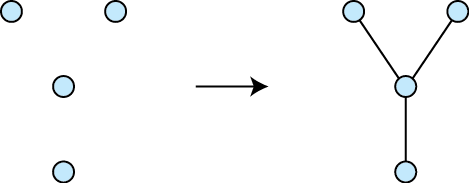
\includegraphics[scale=.75]{CW_Y}
\label{fig:cw_y}
\end{figure}

Since this CW complex is composed of only $1$- and $0$-cells, it will be one-dimensional. If we wished to expand this CW complex, we can take the product of $\Y$ with itself in order to form the product CW complex, which we will illustrate in the following chapter.

While the actual definition of a CW complex still evades us, our interest lies in their application and so we will exchange rigor for convenience as we begin to apply our newfound mathematical tools to building a movement space for robots.
\chapter{Constructing the Configuration Space}

\section{Defining Configuration Space}\label{sec:productspace}

We again turn our attention to the example of the CW complex we just introduced. This ``Y-graph", which we denote as $\Y$, is the simplest non-trivial example of restricted network of robot movement. Other simple graphs have trivial solutions.

\begin{figure}[h]\label{fig:trivial}
\centering
\caption{Examples of Graphs with Trivial Solutions}
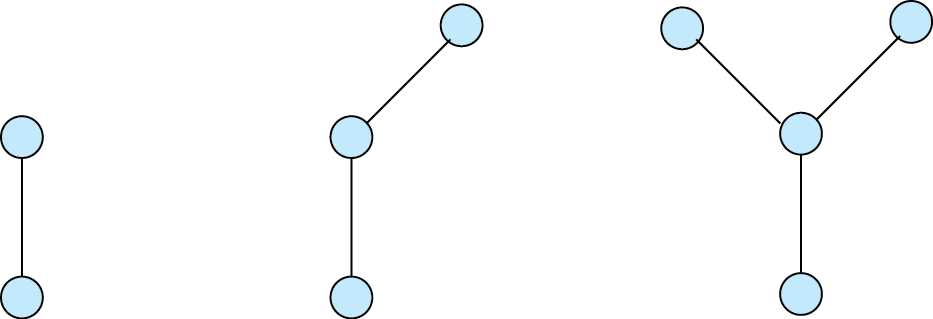
\includegraphics[scale=.5]{Building_Y.png}
\end{figure}


Consider the graph of two vertices connected by an edge as illustrated in Figure~\ref{fig:trivial}. If we have only two robots on this graph, then each of them cannot reach the opposite vertex without collision. Thus, we will attach an additional edge and vertex. However, we again encounter the same problem, so we attach another vertex and edge. Thus we obtain $\Y$. 

\begin{figure}[h]
\caption{The Graph $\Y$}
\centering
\begin{tikzpicture}
  [scale=.7,auto=left,every node/.style={circle,fill=blue!30}]
  \node (n1) {a};
  \node (n2) [above right of=n1]  {b};
  \node (n3) [above left of=n1] {c};
  \node (n4) [below of=n1] {d};

\foreach \from/\to in
{n1/n3,n2/n1,n4/n1}
    \draw (\from) -> (\to);
\end{tikzpicture}
\label{fig:maze}
\end{figure}

So that we may have an interesting problem, we choose to work with $\Y$ as labeled in Figure~\ref{fig:maze}. When there is one robot moving about $\Y$ the solution is trivial since there is nothing for the robot to collide with. It is only when we add an additional robot that things become interesting. 

\begin{defn}
Given a space $X$ with $N$ robots, the configuration space, $C^N(X)$ is defined as $C^N(X)= (\underbrace{X \times X\times \dots \times X}_{N \text{ times} }) - \Delta$ where $$\Delta = \{(x_1, x_2, \dots, x_N) \in X | x_i =x_j \text{ for some } i \neq j\}.$$ 
\end{defn}

Each point in the configuration space $C^N(X)$ is a distinct configuration of $N$ robots at distinct points in $X$, where the robots are labeled $1$, $2$, $\ldots$, $N$ so that $x_i$ is the position of robot $i$ in the space $X$. 

Let us consider two robots which can only move backwards and forwards in a straight line. For these robots, their movement space is $\R$. Thus their configuration space is $C^2(\R) = [\R\times \R]- \{(x_1,x_2)\in \R | x_1 = x_2\}$. Clearly the first part of the configuration space is the plane $\R^2$ where each point represents our two robots' positions on $\R$. The point $(1,3)$, for instance, would mean that robot one is at position one and robot two is at position three in $\R$. However, to obtain our configuration space, we must remove $\Delta$. What are the points in the movement space which represent a collision? They are the points where $x_1=x_2$, and so for this example, they are all the points on the line $y=x$. Thus, removing $\Delta$ ensures that the points in the configuration space are positions where the two robots cannot collide in $\R$.

\begin{figure}[h]\label{fig:xygraph}
\centering
\caption{$C^2(\R)$}
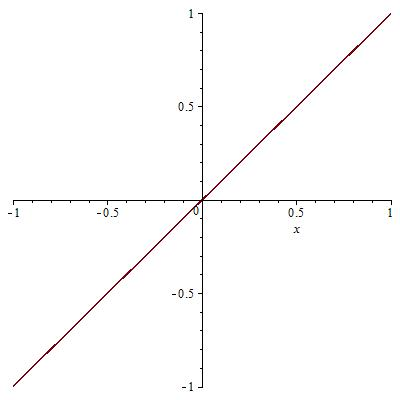
\includegraphics[scale=.25]{Presentation/xygraph.jpg}
\end{figure}



Each time we introduce a new robot to our space we must take another product of their movement space. Adding a new robot to our previous example would yield $C^3(\R)=\R^3 - \{(x_1,x_2,x_3)\in \R^3|x_i=x_j \text{ for some } i \neq j\}$. 

The configuration space $C^2(\R)$, as seen in Figure~
\ref{fig:xygraph} is easy to visualize, but we include it in order to give us a solid foundation when we consider more complicated spaces. Consider, for example,  robots which may move around freely in two-dimensions, such as self-driving cars. The configuration space of two self-driving cars moving around a flat open field would be $C^2(\R^2)= [\R^2 \times \R^2]-\Delta$. As we can see, the problem of collision avoidance quickly escapes our ability to visualize even the simplest non-trivial case and so obscures solutions from our intuition. 

We, however, are not interested with robots moving around a flat plane. Considerable work has been done on this problem. For more information about provably safe configuration spaces we refer readers to Koditschek and Rimon \cite{safe}. Our interest lies in finite networks, such as tracks or guided wires, which robots can move around. As a result, we will examine $\Y$ and its configuration space.

The examples of robots moving about $\R^2$ is hard to visualize, but not necessarily hard to construct. We have been working with $\R^2$ for years and so many of us have a good grasp on the space's properties, but this is not the case for $\Y$. We will construct $C^2(\Y)$ through CW complexes, but we will proceed carefully due to the complexity involved. Recall that the configuration space is defined as $C^2(\Y)~=~(Y\times Y)~-~\Delta$. We begin constructing the configuration space by first building the product space $\Y \times \Y$.

\section{Building the Product Space}

From Chapter 2, we know that graphs are one-dimensional CW complexes composed of $0$ and $1$ cells. The product space of two one-dimensional CW-complexes is a two-dimensional CW-complex, and so to construct the product CW-complex we take the cross product of each cell in the first complex with each cell in the second complex. In the graph $\Y$, we have the $0$-cells $a,b$ and the one cell $(a,b)$. To demonstrate the process for constructing $\Y \times \Y$, let us take the product space of the CW complexes below. Note the subscript on each vertex denotes the position of the first and second robot. 

\begin{figure}[h]
\caption{A Subgraph of $\Y$.}\label{fig:subgraph}
\centering
\begin{tikzpicture}
  [scale=.7,auto=left,every node/.style={circle,fill=blue!30}]
  \node (n1) {$a$};
  \node (n2) [above right of=n1]  {$b$};
  \node (n3) [above left of=n1] {$c$};
  \foreach \from/\to in
{n1/n2, n1/n3}
    \draw (\from) -> (\to);
\end{tikzpicture}
\hspace{1in}
\begin{tikzpicture}
  [scale=.7,auto=left,every node/.style={circle,fill=blue!30}]
  \node (n1) {$a_1$};
  \node (n2) [above right of=n1]  {$b_1$};

\foreach \from/\to in
{n1/n2}
    \draw (\from) -> (\to);
\end{tikzpicture}
\begin{tikzpicture}
  [scale=.7,auto=left,every node/.style={circle,fill=blue!30}]
  \node (n1) {$a_2$};
  \node (n2) [above right of=n1]  {$c_2$};

\foreach \from/\to in
{n1/n2}
    \draw (\from) -> (\to);
\end{tikzpicture}
\end{figure}

We will begin by considering the subgraph of $\Gamma_{Y}$ represented in the left side of Figure~\ref{fig:subgraph}. Let robot one be interested in only moving between positions $a$ and $b$ and let robot two only be interested in moving between positions $a$ and $c$. We represent this visually by the right-hand side of Figure~\ref{fig:subgraph}. We label each vertex by the robot which could be on it, thus $a_1$ is the point where robot one is at position $a$ and $c_2$ is the point where robot two is at position $c$. We should be careful to note that even though we choose to represent our graph in this way in order to simplify the construction of the product $2$-cell, $a_1$ and $a_2$ both represent the same vertex.

To construct the product space, we will follow a series of steps similar to the construction of CW Complexes in Chapter 2. We begin with the collection of $0$-cells, $X^0$. Since our product space consists of the cross product of $\Y$, our vertices in the product space will be the cross product of the $0$-cells as seen in Figure~\ref{fig:vertexcross}. Each vertex is a configuration of robots on $\Y$. For example, $a_1c_2$ is the point where robot one is at $a$ \textit{and} robot two is at $c$.

\begin{figure}[h]
\caption{Cross Product of Vertices}\label{fig:vertexcross}
\centering
\begin{tikzpicture}
  [scale=.7,auto=left,every node/.style={circle,fill=blue!30}]
  \node (n1) at (1,3)  {$a_1c_2$};
  \node (n2) at (3,3)  {$b_1c_2$};
  \node (n3) at (1,1)  {$a_1a_2$};
  \node (n4) at (3,1)  {$b_1a_2$};


\end{tikzpicture}
\end{figure}

Next we take the cross product of the $0$-cells, $a_1$ and $b_1$, with the $1$-cell $(a_2,c_2)$. This will give us two edges vertically connecting the top and bottom vertices with one another. Doing the opposite operation, taking the cross product of $a_2$ and $c_2$ with $(a_1, b_1)$, will give us the two remaining edges. Together, these edges and vertices form the boundary of the $2$-cell.

\begin{figure}[h]
\caption{Cross Product of Vertices and Edges}\label{fig:crosswithedges}
\centering
\begin{tikzpicture}
  [scale=.7,auto=left,every node/.style={circle,fill=blue!30}]
  \node (n1) at (1,3)  {$a_1c_2$};
  \node (n2) at (3,3)  {$b_1c_2$};
  \node (n3) at (1,1)  {$a_1a_2$};
  \node (n4) at (3,1)  {$b_1a_2$};
\foreach \from/\to in
{n1/n3, n2/n4}
    \draw (\from) -> (\to);

\end{tikzpicture}
\hspace{.5in}
\begin{tikzpicture}
  [scale=.7,auto=left,every node/.style={circle,fill=blue!30}]
  \node (n1) at (1,3)  {$a_1c_2$};
  \node (n2) at (3,3)  {$b_1c_2$};
  \node (n3) at (1,1)  {$a_1a_2$};
  \node (n4) at (3,1)  {$b_1a_2$};

\foreach \from/\to in
{n1/n2, n3/n4, n1/n3, n2/n4}
    \draw (\from) -> (\to);

\end{tikzpicture}
\end{figure}

Intuitively, edges in Figure~\ref{fig:crosswithedges} denote one robot's position between vertices. The edge $(a_1c_2, b_1c_2)$ represents the possible positions of robot one between $a$ and $b$, while robot two remains stationary at $c$.

To finish constructing this product space, we must take the product of both $1$-cells. The space $(a_1,b_1)\times (a_2, c_2)$ is homeomorphic to $B^2$, and so our final space is a closed $2$-cell as seen in Figure~\ref{fig:firsttwocell}. A closed $2$-cell represents all the possible positions of the two robots along two edges. 
 
\begin{figure}[h]
\caption{A Closed $2$-Cell}\label{fig:firsttwocell}
\centering
 \begin{tikzpicture}
  [scale=.7,auto=left,every node/.style={circle,fill=blue!30}]
  \node (n1) at (1,3)  {$a_1c_2$};
  \node (n2) at (3,3)  {$b_1c_2$};
  \node (n3) at (1,1)  {$a_1a_2$};
  \node (n4) at (3,1)  {$b_1a_2$};

\foreach \from/\to in
{n1/n2, n3/n4, n1/n3, n2/n4}
    \draw (\from) -> (\to);
    \path[fill=blue!50,opacity=.5] (n1.center) to (n2.center) to (n4.center) to (n3.center) to (n1.center);
\end{tikzpicture}
\end{figure}

We can do this again with the $1$-cells $(a_1,d_1)$ and $(a_2, c_2)$ and obtain its product, seen in Figure~\ref{fig:secondcross}, and then we attach it to the $2$-cell in Figure~\ref{fig:firsttwocell} at the corresponding vertices and edges, which gives us the CW-complex in Figure~\ref{fig:firstattaching}. We may then add the $2$-cell formed by $(a_1, d_1) \times (a_2, b_2)$ to form Figure~\ref{fig:thirdattaching}. If we continue this process without crossing any of the $1$-cells with themselves, we will obtain Figure~\ref{fig:base}.

\begin{figure}[h]
\caption{Cross Product of  $(a_1, d_1)$ and $(a_2,c_2)$}\label{fig:secondcross}
\centering
 \begin{tikzpicture}
  [scale=.7,auto=left,every node/.style={circle,fill=blue!30}]
  \node (n1) at (1,3)  {$a_1c_2$};
  \node (n2) at (3,3)  {$d_1c_2$};
  \node (n3) at (1,1)  {$a_1a_2$};
  \node (n4) at (3,1)  {$d_1a_2$};

\foreach \from/\to in
{n1/n2, n3/n4, n1/n3, n2/n4}
    \draw (\from) -> (\to);
    \path[fill=blue!50,opacity=.5] (n1.center) to (n2.center) to (n4.center) to (n3.center) to (n1.center);
\end{tikzpicture}
\end{figure}



\begin{figure}[h]
\caption{Attached $2$-Cells}\label{fig:firstattaching}
\centering
 \begin{tikzpicture}
  [scale=.7,auto=left,every node/.style={circle,fill=blue!30}]
  \node (n1) at (1,2)  {$b_1a_2$};
  \node (n2) at (1,4)  {$b_1c_2$};
  \node (n3) at (3,1)  {$a_1a_2$};
  \node (n4) at (3,3)  {$a_1c_2$};
  \node (n5) at (5,4)  {$d_1c_2$};
  \node (n6) at (5,2)  {$d_1a_2$};


\foreach \from/\to in
{n1/n3, n2/n4, n1/n2, n4/n3, n4/n5, n5/n6, n6/n3}
    \draw (\from) -> (\to);
    \path[fill=blue!50,opacity=.5] (n1.center) to (n2.center) to (n4.center) to (n3.center) to (n1.center);
    \path[fill=blue!50,opacity=.5] (n4.center) to (n5.center) to (n6.center) to (n3.center) to (n4.center);
\end{tikzpicture}
\end{figure}



\begin{figure}[h]
\caption{Three Attached $2$-Cells}\label{fig:thirdattaching}
\centering
 \begin{tikzpicture}
  [scale=1,auto=left,every node/.style={circle,fill=blue!30}]
  \node (n1) at (1,0)    {$b_1a_2$};
  \node (n2) at (0,2)    {$b_1c_2$};
  \node (n3) at (3,0)    {$a_1a_2$};
  \node (n4) at (1.8,2)  {$a_1c_2$};
  \node (n5) at (3,4)    {$d_1c_2$};
  \node (n6) at (4.2,2)  {$d_1a_2$};
  \node (n7) at (6,2)    {$d_1b_2$};
  \node (n8) at (5,0)    {$a_1b_2$};

\foreach \from/\to in
{n1/n3, n2/n4, n1/n2, n4/n3, n4/n5, n5/n6, n6/n3, n6/n7, n7/n8, n8/n3}
    \draw (\from) -> (\to);
    \path[fill=blue!50,opacity=.5] (n1.center) to (n2.center) to (n4.center) to (n3.center) to (n1.center);
    \path[fill=blue!50,opacity=.5] (n4.center) to (n5.center) to (n6.center) to (n3.center) to (n4.center);
    \path[fill=blue!50,opacity=.5] (n3.center) to (n6.center) to (n7.center) to (n8.center) to (n3.center);
\end{tikzpicture}
\end{figure}



\begin{figure}[h]
\caption{Six Attached $2$-Cells}\label{fig:base}
\centering
 \begin{tikzpicture}
  [scale=1,auto=left,every node/.style={circle,fill=blue!30}]
  \node (n1) at (1,0)       {$b_1a_2$};
  \node (n2) at (0,2)       {$b_1c_2$};
  \node (n3) at (3,0)       {$a_1a_2$};
  \node (n4) at (1.8,2)     {$a_1c_2$};
  \node (n5) at (3,4)       {$d_1c_2$};
  \node (n6) at (4.2,2)     {$d_1a_2$};
  \node (n7) at (6,2)       {$d_1b_2$};
  \node (n8) at (5,0)       {$a_1b_2$};
  
  \node (n9) at (0,-2)      {$b_1d_2$};
  \node (n10) at (1.8, -2)  {$a_1d_2$};
  \node (n11) at (3,-4)     {$c_1d_2$};
  \node (n12) at (4.2, -2)  {$c_1a_2$};
  \node (n13) at (6,-2)     {$c_1b_2$};

\foreach \from/\to in
{n1/n3, n2/n4, n1/n2, n4/n3, n4/n5, n5/n6, n6/n3, n6/n7, n7/n8, n8/n3, n1/n9, n9/n10, n10/n3, n10/n11, n11/n12, n12/n3, n12/n13, n13/n8}
    \draw (\from) -> (\to);
    \path[fill=blue!50,opacity=.5] (n1.center) to (n2.center) to (n4.center) to (n3.center) to (n1.center);
    \path[fill=blue!50,opacity=.5] (n4.center) to (n5.center) to (n6.center) to (n3.center) to (n4.center);
    \path[fill=blue!50,opacity=.5] (n3.center) to (n6.center) to (n7.center) to (n8.center) to (n3.center);
    \path[fill=blue!50,opacity=.5] (n1.center) to (n9.center) to (n10.center) to (n3.center) to (n1.center);
    \path[fill=blue!50,opacity=.5] (n3.center) to (n10.center) to (n11.center) to (n12.center) to (n3.center);
    \path[fill=blue!50,opacity=.5] (n3.center) to (n12.center) to (n13.center) to (n8.center) to (n3.center);
\end{tikzpicture}
\end{figure}

But we are not yet finished. We must now cross all the $1$-cells with themselves. This is where our space becomes messy. In order to visualize this, we will embed the product space in $\R^3$. Figure \ref{fig:productspace} represents all possible moves two robots may make, regardless of whether or not a collision will occur. Since there are three $1$-cells and four $0$-cells in $\Y$, our final product space will consist of $9$ $2$-cells, twenty-four $1$-cells, and sixteen $0$-cells.

\begin{figure}[h]
\caption{$\Y \times \Y$}\label{fig:productspace}
\centering
 \begin{tikzpicture}
  [scale=1,auto=left,every node/.style={circle,fill=blue!30}]
  \draw[thick,->,black] (-7,0,0) -- (7,0,0) node[anchor=north east]{$y$};
  \draw[thick,->] (0,0,0) -- (0,7,0) node[anchor=north east]{$z$};
  \draw[thick,->] (0,0,7) -- (0,0,-7) node[anchor=east]{$x$};
  
  \node (n0) at (0,0,0)         {$a_1a_2$};
  \node (n1) at (0,0,-5)        {$d_1c_2$};
  \node (n2) at (0,0,6)         {$c_1d_2$};
  \node (n3) at (-3,0,0)        {$b_1a_2$};
  \node (n4) at (3,0,0)         {$a_1b_2$};
  \node (n5) at (-4,0, 2)       {$b_1d_2$};
  \node (n6) at (-2,0, 3)       {$a_1d_2$};
  \node (n7) at (-4,0,-3)       {$b_1c_2$};
  \node (n8) at (-2,0,-3)       {$a_1c_2$};
  \node (n9) at (2,0, 3)        {$c_1a_2$};
  \node (n10) at (5, 0, 3)      {$c_1b_2$};
  \node (n11) at (3.5, 0, -3)   {$d_1b_2$};
  \node (n12) at (2, 0, -3)     {$d_1a_2$};
  \node (n13) at (0, 6, 0)      {$d_1d_2$};
  \node (n14) at (0, 4, 0)      {$c_1c_2$};
  \node (n15) at (0,2,0)        {$b_1b_2$};
  
  \foreach \from/\to in
{n0/n8, n0/n9, n0/n6, n0/n12, n0/n3, n0/n4, n4/n11, n11/n12, n4/n10, n10/n9, n12/n1, n1/n8, n8/n7, n7/n3, n3/n5, n5/n6, n6/n2, n2/n9, n6/n13, n13/n12, n8/n14, n14/n9, n3/n15, n15/n4}
    \draw (\from) -> (\to);
    \path[fill=blue!50,opacity=.5] (n1.center) to (n12.center) to (n11.center) to (n4.center) to (n10.center) to (n9.center) to (n2.center) to (n6.center) to (n5.center) to (n3.center) to (n7.center) to (n8.center) to (n1.center);
    \path[fill=blue!50,opacity=.5] (n6.center) to (n13.center) to (n12.center) to (n6.center);
    \path[fill=blue!50,opacity=.5] (n8.center) to (n14.center) to (n9.center) to (n8.center);
    \path[fill=blue!50,opacity=.5] (n3.center) to (n15.center) to (n4.center) to (n3.center);
\end{tikzpicture}
\end{figure}
\clearpage

\newpage

\newpage
\section{The Configuration Space}

Now that we have the product space of $\Y \times \Y$, we must remove the pairwise diagonal $\Delta$ to complete the construction of the configuration space $C^2(\Y)$. Recall that $\Delta = \{(x_1,x_2,\dots, x_n)\in X | x_i = x_j\text{ for some } i \neq j\}$.

Let us consider the $2$-cell formed by $(a_1b_1)\times (a_2b_2)$ as pictured in Figure~\ref{fig:twosaywhat}. The $0$-cells $a_1a_2$ and $b_1b_2$ are both points where both robots collide on the same vertex. In addition to colliding at a vertex, both robots may move, and hence collide, along the edge connecting $a$ and $b$. As a result, we must also remove this space, represented by the diagonal line, from our configuration space. 

\begin{figure}[h]
\caption{The $2$-cell Formed by $(a_1b_1)\times (a_2b_2)$ }\label{fig:twosaywhat}
\centering
 \begin{tikzpicture}
  [scale=.7,auto=left,every node/.style={circle,fill=blue!30}]
  \node (n1) at (1,3)  {$a_1b_2$};
  \node (n2) at (3,3)  {$b_1b_2$};
  \node (n3) at (1,1)  {$a_1a_2$};
  \node (n4) at (3,1)  {$b_1a_2$};

\foreach \from/\to in
{n1/n2, n3/n4, n1/n3, n2/n4}
    \draw (\from) -> (\to);
    \path[fill=blue!50,opacity=.5] (n1.center) to (n2.center) to (n4.center) to (n3.center) to (n1.center);
\end{tikzpicture}
\hspace{.5in}
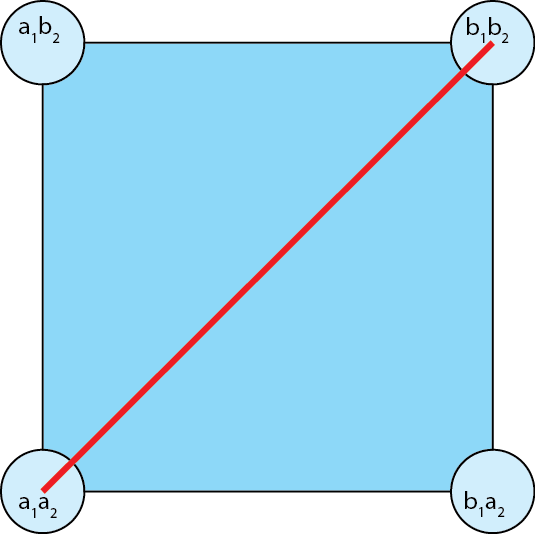
\includegraphics[scale=.3]{Export.png}
\end{figure}

Repeating this process for every other $2$-cell obtained by taking the product of a $1$-cell with itself and putting the configuration space together, we obtain Figure~\ref{fig:config}. The dotted lines are used to represent where a pairwise diagonal element was removed.

\begin{figure}[h]
\centering
\caption{$C^2(\Y)$ [Arb00]}
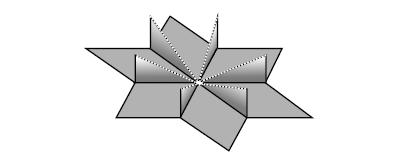
\includegraphics[scale=1]{Presentation/Config.jpg}
\label{fig:config}
\end{figure}

This is the configuration space of $C^2(\Y)$. While it is easier to visually intuit, this configuration space for two robots is already embedded in the three dimensional space $R^3$. For more robots, our ability to draw these configuration spaces quickly escapes us. Thus we will employ topological tools to simplify the dimension of the space into something more tractable.
\chapter{Discretizing the Configuration Space}
The ability to construct the configuration space for two robots on $\Y$ is important, but it is not all that immediately useful. Robots move around a fixed movement network in order to carry out tasks, but they are not autonomous; they need to be scheduled. In order to create efficient movement schemes, robotic engineers commonly employ algorithms from graph theory.

Unfortunately, these algorithms do not generally work well on configuration spaces. When additional robots are introduced to a movement network, the dimension of the network's configuration space will increase. As a result, the algorithms employed to find the necessary configurations for robots to reach their destinations become increasingly inefficient. 

Thus it is necessary to simplify the dimension of our configuration spaces through a process known as discretization. By removing elements of a configuration space, we reduce its complexity so that we may apply the necessary algorithms. A simplified configuration space is called the \textbf{discretized configuration space}.


\begin{defn}
The discretized configuration space, $\mathcal{D}^N( X)$, is defined as $$\mathcal{D}^N(X) = (\underbrace{X\times X \times \dots \times X}_{N\text{ times}}) - \tilde{\Delta} $$ where $\tilde{\Delta}$ is the collection of all cells whose closure intersects the pairwise diagonal. The closure of an n-cell is the corresponding closed n-cell.
\end{defn}

To demonstrate the definition of a configuration space will discretize \C.


\begin{figure}[h]
\centering
\caption{$C^2(\Y)$}
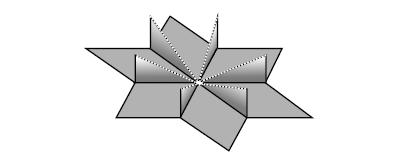
\includegraphics[scale=1]{Presentation/Config.jpg}
\label{fig:config4}
\end{figure}

Let us take a moment to fully explore the implications of $\tilde{\Delta}$'s definition in the context of two robots on $\Y$. Notice the missing central vertex and dashed lines in Figure~\ref{fig:config4}. Every cell whose closure intersects either the dashed line or central vertex representing the pairwise diagonal must be removed. For this specific discretization, we remove cells which intersect the boundary by visually identifying them, and then removing them from our space. To illustrate, we will discretize the $2$-cell in Figure~\ref{fig:d_2cell}.

\begin{figure}[h]
\centering
\caption{Discretizing a $2$-cell from \C.}
\vspace{2mm}
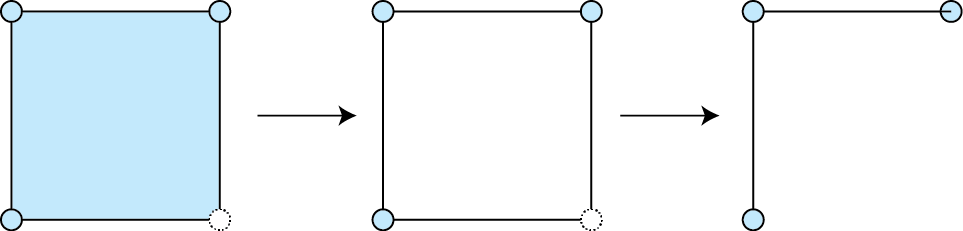
\includegraphics[scale=.8]{2_Cell_Example.png}
\label{fig:d_2cell}
\end{figure}

We begin by identifying the cells whose closure intersects the pairwise diagonal. The notion of closure has an explicit meaning in topology which would require an excessive amount of background material. Hence, we will only discuss closure in the context of CW complexes. We can intuitively conceptualize the closure of a CW-complex as a closed $n$-cell. Thus, when we discretize a space, we must remove all $n$-cells which are not closed. We know the closure of a closed $2$-cell is a $2$-cell along with the attached $1$-cells which form its boundary. Since we have removed a section of the closed $2$-cell's boundary, the $2$-cell is not closed and so it must be removed. We are left with our attached $1$-cells, but not all of these $1$-cells are closed, and so we must also remove them. Thus we are left with a discretized $2$-cell. Doing so for every CW complex in \C will give us $\mathcal{D}^2(\Y)$ as pictured in Figure~\ref{fig:star}.

\begin{figure}[h]
\centering
\caption{$\mathcal{D}^2(\Y)$}

\includegraphics[scale=.5]{discretized.png}
\label{fig:star}
\end{figure}

This process is called discretization. For spaces such as $C^2(\Y)$, it may be simple to discretize by visually evaluating the configuration space and removing all cells which belong to $\tilde{\Delta}$. Yet as we have seen, the dimension of a configuration space increases rapidly with each additional robot, and so discernible graphs for more complex spaces are extremely rare. 

In order to emancipate ourselves from visual tools, we will form the discretized configuration space through a series of deformation retracts. Retracting $C^2(\Y)$ to $\mathcal{D}^2(\Y)$ is done by first retracting the punctured closed $2$-cells onto their respective boundaries, and then retracting all punctured closed $1$-cells onto their respective boundaries. The remainder of this chapter will carefully illustrate this process.

In order to retract all $2$-cells of $C^2(\Y)$ we must first define the deformation retract. This subset of our configuration space is the $n$-skeleton.

The $2$-skeleton is the collection of $1$-cells and $0$-cells as seen in Figure~\ref{fig:noint}. Now that we have selected a deformation retract, we now define a retraction for each $2$-cell. 

\begin{figure}[h]
\centering
\caption{$n$-Skeleton of $C^2(\Y)$}
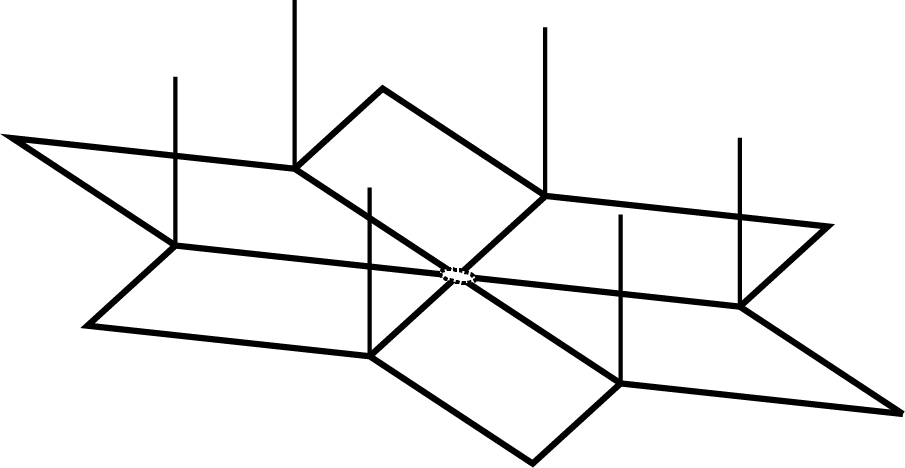
\includegraphics[scale=.5]{NoInt.png}
\label{fig:noint}
\end{figure}


We know the closed $2$-cell to be homeomorphic to the closed ball of dimension two, so it suffices to show that there exists a retraction from the closed two-dimensional ball to the unit circle. Unfortunately, it can be shown that no such retraction exists\cite{retract}. Thankfully, the union of our $2$-cells and their boundaries is not actually closed. Looking back to Figure~\ref{fig:config4}, we see that every closed $2$-cell intersects at least one point of the pairwise diagonal, so our closed $2$-cells are actually punctured closed balls with the puncture on the boundary of the $2$-cell.

This critical property of our configuration space allows us to retract every closed $2$-cell onto its boundary. While it is possible to explicitly define these retractions, we refrain from doing so due to time constraints.

\begin{figure}[h]
\centering
\caption{The Deformation Retract of a Punctured Ball to its Boundary}
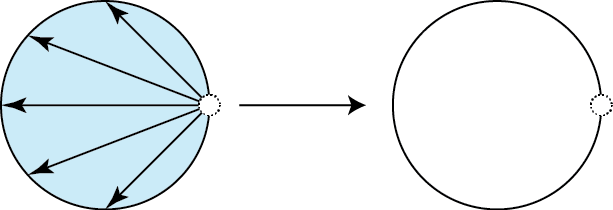
\includegraphics[scale=1]{PuncturedBall.png}
\label{fig:pball}
\end{figure}

Figure~\ref{fig:pball} demonstrates the retraction given by $$F\colon D^2\setminus \{p\}\times I \rightarrow D^2\setminus \{p\},$$ where $\{p\}$ denotes the puncture. 

In order to aid our intuition, imagine a punctured closed ball as pictured on the left-hand side of Figure~\ref{fig:pball} with a very tiny balloon inserted at the point of puncture. We then inflate the balloon until it completely fills the sphere. This example illustrates how the $2$-cell is retracted onto its boundary. 

We should note, however, that additional restrictions apply. Since $2$-cells share boundaries, every point in a $2$-cell will have a ``twin'' in each $2$-cell that shares its boundary. These  must be mapped to the analogous boundary point \textit{simultaneously}. Figure~\ref{fig:twins} demonstrates this for attached $2$-cells. 


\begin{figure}[ht]
\centering
\caption{A Simultaneous Twin Retraction in Attached $2$-Cells}
\vspace{3mm}
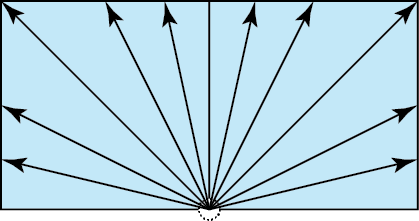
\includegraphics[scale=1]{Twins.png}
\label{fig:twins}
\end{figure}

While we have been describing $F$ for $1$- or $2$-cells, all cells in the configuration space must be continuously and simultaneously retracted onto their respective boundaries. This retraction will yield the $2$-skeleton. 

Let us consider the significance of the $2$-skeleton. Each $2$-cell represents the configuration where both robots are simultaneously on edges. Since we have removed these cells, only one robot is allowed to move between vertices of $\Y$ while the other robot is forced to wait at a vertex.

We now retract the remaining cells of $\tilde{\Delta}$ onto their boundaries. These cells are the punctured $1$-cells of the $2$-skeleton. We retract the puncutured $1$-cells by drawing them into their boundary. Formally, our second retraction, $G$, is given by $G\colon D^1\setminus\{p\} \times I \rightarrow D^1\setminus\{p\} $. Similarly to the first retraction, each $1$-cell must be continuously and simultaneously retracted onto its boundary. Performing this deformation retract yields the discretized configuration space as seen in Figure~\ref{fig:disc}.


\begin{figure}[h]
\caption{$\mathcal{D}^2(\Y)$}\label{fig:disc}
\centering
 \begin{tikzpicture}
  [scale=1,auto=left,every node/.style={circle,fill=blue!30}]
  \node (n1) at (1,0)       {$b_1a_2$};
  \node (n2) at (0,2)       {$b_1c_2$};
  \node (n4) at (1.8,2)     {$a_1c_2$};
  \node (n5) at (3,4)       {$d_1c_2$};
  \node (n6) at (4.2,2)     {$d_1a_2$};
  \node (n7) at (6,2)       {$d_1b_2$};
  \node (n8) at (5,0)       {$a_1b_2$};
  
  \node (n9) at (0,-2)      {$b_1d_2$};
  \node (n10) at (1.8, -2)  {$a_1d_2$};
  \node (n11) at (3,-4)     {$c_1d_2$};
  \node (n12) at (4.2, -2)  {$c_1a_2$};
  \node (n13) at (6,-2)     {$c_1b_2$};

\foreach \from/\to in
{ n2/n4, n1/n2,  n4/n5, n5/n6, n6/n7, n7/n8, n1/n9, n9/n10, n10/n11, n11/n12, n12/n13, n13/n8}
\draw (\from) -> (\to);
\end{tikzpicture}
\end{figure}

As we can see from the illustration above, retracting \C produces $\mathcal{D}^2(\Y)$. Having obtained the discretized configuration space, it is now possible to apply algorithms to determine optimal movement schemes.

Over the course of this chapter we have treated the discretization of the configuration space as two separate operations, but this is inelegant. If we define another homotopy $H\colon C^2(\Y)\times I \rightarrow C^2(\Y)$ such that $H(x,0)=F(x,0)$, $H(x,\frac{1}{2}) = F(x,1) = G(x,0)$, and $H(x,1)=G(x,1)$, we can retract the configuration space in one step.

While we are able to neatly demonstrate discretization through deformation retracts for $C^2(\Y)$, we will see in the next chapter that not all spaces behave so nicely.

\chapter{Conditions of Discretization}
In the previous chapter, retracting the configuration space yielded connected discretized configuration space, however, not all spaces behave so nicely. This chapter will first examine examples of robot movement networks which do not discretize well, and then present a method for determining which graphs have a configuration space that can be discretized using a deformation retract.

\section{When Deformation Retracts are Successful}
Whenever we discretize a configuration space we eliminate portions of it, thus losing information. In the case of \C, this was a benefit as it simplified a provably safe configuration space into a more tractable one. Whenever we make a space finer, we risk losing necessary properties of our space. 

In order to demonstrate, we will discretize the two robot configuration space of the graph seen in Figure~\ref{fig:bad}, which we will call $\Gamma_{\Psi}$. Unlike $\Y$, the graph $\Gamma_{\Psi}$ contains a cycle, and so its paths need not be unique. It is these properties which will not allow us to nicely discretize its configuration space. 

\begin{figure}[h]
\centering
\caption{The Graph $\Gamma_{\Psi}$}
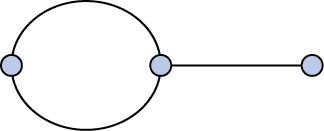
\includegraphics[scale=1]{Bad.png}
\label{fig:bad}
\end{figure}

It can be shown using a process similar to that in Chapter 3, that the configuration space for two robots on $\Gamma_{\Psi}$, denoted by $C^2(\Gamma_{\Psi})$, yields the configuration space in Figure~\ref{fig:C_Psi}.

\begin{figure}[h]
\centering
\caption{$C^2(\Gamma_{\Psi})$\cite{factory}}
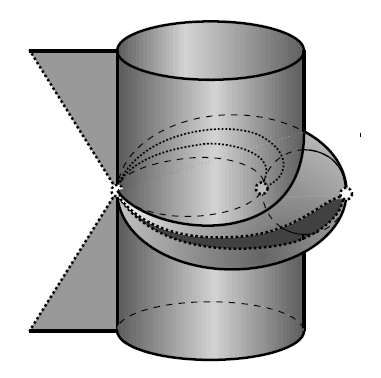
\includegraphics[scale=.5]{Bad_C.png}
\label{fig:C_Psi}
\end{figure}

Here we again see the complexity that arises when working with configuration spaces. Even though $\Gamma_{\Psi}$ seems simpler than $\Y$, its configuration space is much harder to visualize. This becomes even more apparent when we attempt to simplify $C^2(\Gamma_{\Psi})$ in order to obtain the discretized configuration space $\mathcal{D}^2(\Gamma_{\Psi})$. 

\begin{figure}[h]
\centering
\caption{$\mathcal{D}^2(\Gamma_{\Psi})$}
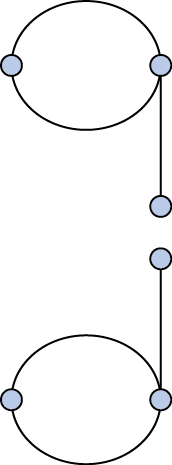
\includegraphics[scale=.5]{Bad_D.png}
\label{fig:D_Psi}
\end{figure}

The graph in Figure~\ref{fig:D_Psi} is the discretized configuration space $\mathcal{D}^2(\Gamma_{\Psi})$. Unlike $\mathcal{D}^2(\Y)$, this space cannot be used to simplify robot movement schedules. Since $\mathcal{D}^2(\Gamma_{\Psi})$ is not connected, half of the possible position configurations will be excluded depending on the initial configuration of the two robots. This renders algorithms used to find optimal movement schemes useless. 

While we can easily obtain the discretized configuration spaces for the relatively simple configuration spaces of \C and $C^2(\Gamma_{\Psi})$ by visually discretizing, this may not be the case for more complicated movement networks. The previous chapter illustrated a method for generally discretizing a configuration space by demonstrating a deformation retract on \C. In order for a space to be nicely discretizable by a deformation retract, it must meet the conditions of Theorem~\ref{thm:when}

\begin{thm}\label{thm:when}
For any $N$ robots with $N>1$, on a graph $\Gamma$ with at least $N$ vertices, $C^N(\Gamma)$ retracts onto $D^N(\Gamma)$ if and only if 

\begin{enumerate}
\item Each path between distinct essential vertices passes through at least $N-1$ edges; and,
\item Each cycle not homotopic to a point passes through at least $N+1$ edges.\cite{factory}
\end{enumerate}
\end{thm}

We know that $\Gamma_{\Psi}$ contains a cycle. Since the cycle consists of two attached $1$-cells, it cannot be retracted to a point for the same reason a closed $2$-cell cannot be retracted onto its boundary. Thus $C^2(\Gamma_{\Psi})$ cannot be nicely discretized because the cycle which is not homotopic to a point passes through only two edges and hence does not satisfy Condition 2 of Theorem~\ref{thm:when}.

Discretizing \C  yields a CW complex of dimension one, which we know is a graph from Chapter 3. As a result, algorithms from graph theory can be used to find optimal series of configurations for two robots to navigate a graph. Additionally, the following theorem states the the maximum dimension of the discretized configuration space is dependant on the number of vertices with degree greater than two in the movement network.

\begin{thm} \label{thm:dim}
Given a graph $G$ with $V$ vertices of degree greater than two, the discretization of $C^N(G)$ has a dimension of at most $V$.~\cite{factory}
\end{thm}

Abrams and Ghrist also show that by incorporating Theorem~\ref{thm:dim}, one can control the dimension, and therefore computational complexity, of the discretized configuration space\cite{factory}. This theorem deserves note because it allows robotic engineers to design movement schemes with the dimension of the discretized configuration space in mind. Thus we can know how to construct discretizable movement networks, build their configuration spaces, and then retract them to form their discretized forms.

We have shown that $\Y$ discretizes to a CW complex of dimension one, but we can extend this to all graphs which have radial vertices connecting a central vertex. Explicitly, we say $\Y = \Upsilon_3$, where $\Upsilon_N$ is a graph of $N-1$ vertices which are only adjacent to a central vertex. Thus every movement network belonging to $\Upsilon_N$ will discretize to a one-dimensional CW complex.

Together, Theorems~\ref{thm:when} and~\ref{thm:dim} allow robotic engineers to design movement networks which will always discretize nicely while controlling for their complexity. As a result, the configuration and discretized configuration spaces of fixed movement networks such as $\Gamma_{\Psi}$ need not even be computed. 

\section{Conclusions}
By carefully exploring the discretization of \C, we have demonstrated how the application of topological tools can radically simplify the problem of robotic movement along fixed pathways. Beyond this explicit example however, we hope that readers view this work as a guide to solving future problems pertaining to fixed path movement. 

While we feel this thesis provides a thorough examination of \C 's discretization process, further work could still be done. While we have provided a plausible method for deformation retracting \C onto $\mathcal{D}^2(\Y)$, time has unfortunately left us unable to provide a formal proof for our technique. It is our hope that the deformation retract presented in this paper could be rigorously proven in order to further illustrate discretization techniques. 

Additionally, Abrams points out in his thesis that his proof of \C 's discretization requires further work, because it incorporated Whitehead's theorem, and so we as not completely self-contained~\cite{thesis}. In the article he coauthored with Ghrist, however, he not only seems to solve this problem, but strengthen his theorem~\cite{factory}. Exactly how Abrams and Ghrist manage to strengthen their proofs merits examination which may shed further light on the mechanics involved in Theorems~\ref{thm:when} and \ref{thm:dim}.

The work done here only serves to set up the problem of robotic movement. The impetus for discretizing configuration spaces is that we may apply the tools of graph algorithms to achieve specific robot configurations. We hope that readers use this thesis as an accessible introduction to the topic so that further advancement in the field may occur.


\backmatter
		% Use \include{appendixB} to include another appendix.
\bibliographystyle{unsrt}%Used BibTeX style is unsrt
\bibliography{TheBib}
\end{document}
